\begin{slikaDesno}{fig/pz_koreni_jedinice.pdf}
    \PID 
    Преносна карактеристика реалног дискретног филтра без нула функциjе преноса
    дата jе половима у $z$-равни. Сви полови функциjе преноса се налазе на кружници
    полупречника $r = \dfrac12$, jедан од полова jе реалан, а потег другог заклапа са позитивним
    делом реалне осе угао $\upphi = \dfrac{2\uppi}{3}$, као на слици. Позната jе jош и минимална вредност
    амплитудске фреквенцијске карактеристике $|H(\jj\Omega)|_{\rm min} = 1$. 
    \begin{enumerate}
        \item[(а)]  Одредити функцију
                    преноса филтра $H(z)$, и скицирати његову амплитудску карактеристику у 
                    опсегу дискретних кружних учестаности $0 \leq \Omega \leq \uppi$.
    \end{enumerate}
    Одредити (в) импулсни одзив
\end{slikaDesno}
\begin{enumerate}
    \item[(б)] Одредити импулсни одзив датог филтра, $h[n]$. 
    \item[(в)] Одредити комплетни одзив овог филтра на побуду $x[n] = \cos(\uppi n)\, \uu[n]$
\end{enumerate}

\RESENJE
Полови дефинисани задатком представљају треће корене\footnote{У општем случају, различитих $n$-тих коренова  
броја $z = \uprho \ee^{\jj\uptheta} \in \mathbb C$ има $n$, и дати су изразом 
$\sqrt[n]{z} = \sqrt[n]{\uprho} \exp{\jj k \dfrac{\uptheta + 2\uppi k}{n}}$, где је $k \in \{0,\ldots,n-1\}$.} 
комплексног броја $\dfrac{1}{8}$, односно јесу решење једначине 
$z^3 - \dfrac{1}{8} = 0$. На основу тога, функција преноса посматраног дискретног система може се представити у облику 
$H(z) = H_0 \dfrac{1}{z^3 - \dfrac{1}{8}}$, где је $H_0$ константа коју је потребно одредити.  

Константа се може потражити из другог услова о минималној вредности амплитудске фреквенцијске карактеристике.
Амплитудска фреквенцијска карактеристика дискретног система одређена је као $|H(z)|$ где је 
$ z = \ee^{\jj\Omega}$. На основу тога, даље се има\footnote{
    Користи се идентитет $z z^{\ast} = |z|^2$, $z \in \mathbb C$. Такође се користе и особине комплексне конјукције
    $(z + w)^* = z^* + w^*$ и $(z/w)^* = z^*/w^*$, за $z,w\in\mathbb C$.
}
\begin{eqnarray*}
    |H(z)|^2 &=& \left( H_0 \dfrac{1}{z^3 - \dfrac{1}{8}} \right) \cdot  \left( H_0 \dfrac{1}{z^3 - \dfrac{1}{8}} \right)^*
              =  H_0^2 \dfrac{1}{ \left(z^3 - \dfrac{1}{8}\right)\left((z^3)^* - \dfrac{1}{8}\right)  } 
            \\
             &=& \dfrac{H_0^2}{ \underbrace{(zz^*)^3}_{\mathclap{ |\ee^{\jj\Omega}|^3 = 1 }} - \dfrac{1}{8} 
             \underbrace{\left( (z^3)^* + z^3 \right)}_{2\Re{z^3} = 2\cos(3\Omega) } + \dfrac{1}{64} } 
             = 
             \dfrac{H_0^2}{ 1 + \dfrac{1}{64} - \dfrac{1}{4}\cos(3\Omega) } \Rightarrow \\
    |H(\ee^{\jj\Omega})| &=& \dfrac{H_0}{ \sqrt{ 1 + \dfrac{1}{64} - \dfrac{1}{4}\cos(3\Omega)} }.
\end{eqnarray*}
Минимум амплитудске фреквенцијске карактеристике постиже се за максималну вредност $\cos(3\Omega) = -1$, па је онда 
\begin{eqnarray}
    |H(\ee^{\jj\Omega})|_{\min} &=& \dfrac{H_0}{ \sqrt{ 1 + \dfrac{1}{64} + \dfrac{1}{4} } } = 1 
    \Rightarrow H_0 = \dfrac{9}{8}.
\end{eqnarray}
Дијаграм амплитудске карактеристике представљен је на слици \ref{\ID.fig.H}.
\begin{figure}[ht!]
    \centering
    \begin{subfigure}{0.49\textwidth}
        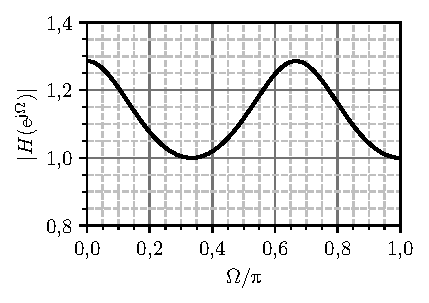
\includegraphics{fig/koreni_plot.pdf}
        \caption{Дијаграм амплитудске фреквенцијске карактеристике филтра}
        \label{\ID.fig.H}    
    \end{subfigure}
    %
    \begin{subfigure}{0.49\textwidth}
        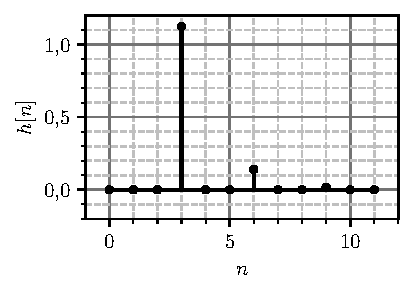
\includegraphics{fig/koreni_h.pdf}
        \caption{Дијаграм импулсног одзива филтра}
        \label{\ID.fig.himp}    
    \end{subfigure}
\end{figure}


(б) Импулсни одзив датог филтра може се одредити растављањем на парцијалне разломке, или алтернативно, 
развојем добијеног израза у степени ред\footnote{ Користи се развој
$\dfrac{1}{1 - q} = \sum_{k = 0}^\infty q^k$, у случају када је $|q| < 1$. } по $z^{-1}$ 
\begin{eqnarray}
    H(z) &=& \dfrac{9}{8} \dfrac{1}{z^3 - \dfrac{1}{8}} =
           \dfrac{9}{8} z^{-3} \dfrac{1}{1 - \underbrace{\dfrac{1}{8}z^{-3}}_q }
         = \dfrac{9}{8} z^{-3} \sum_{k = 0}^{\infty} \left(\dfrac{1}{8}\right)^k z^{-3k} \\
         &=& \dfrac{9}{8} z^{-3} \sum_{k = 0}^{\infty} \left(\dfrac{1}{8}\right)^k z^{-3(k+1)} 
        =  \sum_{m = 1}^{\infty} \dfrac{9}{8}\left(\dfrac{1}{8}\right)^{m-1} z^{-3m},
\end{eqnarray}
при чему је у последњем кораку искоришћена смена $m = k + 1$. 
Овакав развој у ред је оправдан, јер сваки члан реда представља одбирке од којих сваки делује на само један тренутак времена, 
па у том смислу, не постоји проблем са конвергенцијом таквог развоја. Разматрањем финалног израза можемо да уочимо да 
он представља израчунавање $\mathcal{Z}$-трансформације по дефиницији 
$X(z) = \sum_{n = 0}^{\infty} x[n] z^{-n}$. Примећујемо да сигнал има само одбирке у тренуцима $n = 3m$ када је 
одговарајућа вредност $x[n] = \dfrac{9}{8}\left(\dfrac{1}{8}\right)^{m-1}$, другим речима, може се писати 
\begin{equation}
    x[n] = \begin{cases}
        \dfrac{9}{8}\left(\dfrac{1}{8}\right)^{\frac{n}{3}-1} &, 3|n \land n \geq 3 \\
        0 &, \text{иначе}
    \end{cases}.
\end{equation}
